\documentclass{article}
\usepackage{pgfplots}
\usepackage[left=2.5cm,right=2cm,top=2cm,bottom=2cm]{geometry}
\pgfplotsset{compat=1.8}
\usetikzlibrary{patterns}

\begin{document}
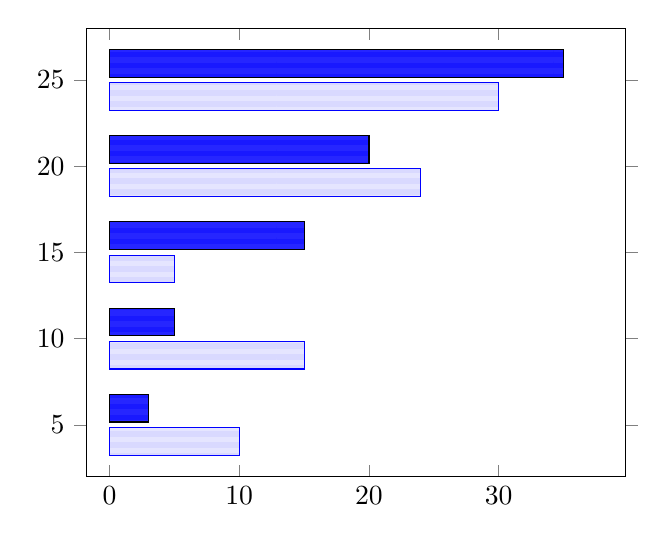
\begin{tikzpicture}
  \begin{axis}[xbar,enlargelimits=0.15] % xbar horizontal bar graph
    \addplot
        [draw=blue,pattern=horizontal lines light blue]
        coordinates
        {(10,5) (15,10) (5,15) (24,20) (30,25)};
        \addplot
            [draw=black,pattern=horizontal lines dark blue]
            coordinates
            {(3,5) (5,10) (15,15) (20,20) (35,25)};
  \end{axis}
\end{tikzpicture}

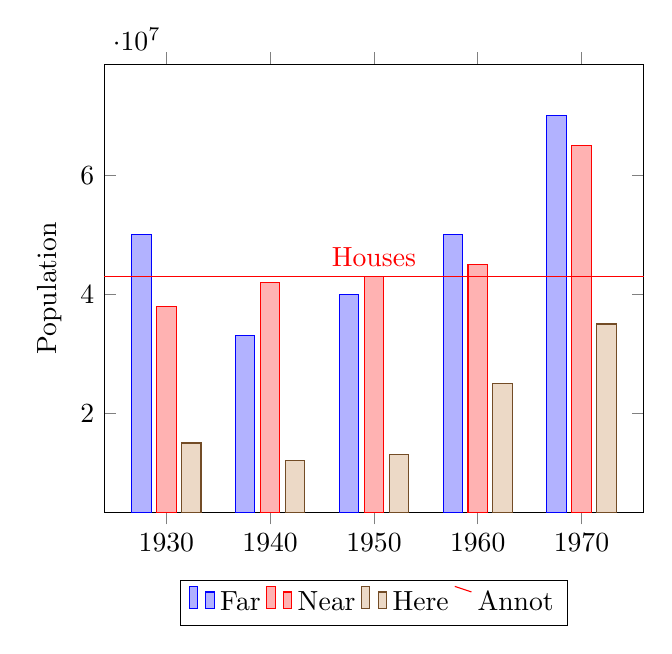
\begin{tikzpicture}
  \begin{axis}[x tick label style={
        /pgf/number format/1000 sep=
      },
      ylabel=Population,
      enlargelimits=0.15,
      legend style={at={(0.5,-0.15)},
        anchor=north,legend columns=-1},
      ybar,
      bar width=7pt,
    ]
    \addplot
    coordinates {(1930,50e6) (1940,33e6)
      (1950,40e6) (1960,50e6) (1970,70e6)};

    \addplot
    coordinates {(1930,38e6) (1940,42e6)
      (1950,43e6) (1960,45e6) (1970,65e6)};

    \addplot
    coordinates {(1930,15e6) (1940,12e6)
      (1950,13e6) (1960,25e6) (1970,35e6)};

    \addplot[red,sharp plot,update limits=false]
    coordinates {(1910,4.3e7) (1990,4.3e7)}
    node[above] at (axis cs:1950,4.3e7) {Houses};

    \legend{Far,Near,Here,Annot}
  \end{axis}
\end{tikzpicture}

% Define bar chart colors
%
\definecolor{bblue}{HTML}{4F81BD}
\definecolor{rred}{HTML}{C0504D}
\definecolor{ggreen}{HTML}{9BBB59}
\definecolor{ppurple}{HTML}{9F4C7C}


\begin{tikzpicture}
  \begin{axis}[
      width  = 0.85*\textwidth,
      height = 8cm,
      major x tick style = transparent,
      ybar=2*\pgflinewidth,
      bar width=14pt,
      ymajorgrids = true,
      ylabel = {Run time speed},
      symbolic x coords={EgyptHD,Hover,Navi},
      xtick = data,
      scaled y ticks = false,
      enlarge x limits=0.25,
      ymin=0,
      legend cell align=left,
      legend style={
        at={(1,1.05)},
        anchor=south east,
        column sep=1ex
      }
    ]
    \addplot[style={bblue,fill=bblue,mark=none}]
    coordinates {(EgyptHD, 1.0) (Hover,1.0) (Navi,1.0)};

    \addplot[style={rred,fill=rred,mark=none}]
    coordinates {(EgyptHD,1.123) (Hover,0.85) (Navi,1.09)};

    \addplot[style={ggreen,fill=ggreen,mark=none}]
    coordinates {(EgyptHD,0.92) (Hover,0.56) (Navi,0.95)};

    \addplot[style={ppurple,fill=ppurple,mark=none}]
    coordinates {(EgyptHD,0.74) (Hover,1.07) (Navi,1.23)};
    \legend{No vectorization,TreeScore $>2$,TreeScore $>3$,TreeScore $>4$}
  \end{axis}
\end{tikzpicture}


\pgfplotstableread{
  3 38.9575
  4 166.897
  6 53.63835
  7 39.6594
  8 82.1631
  9 40.22045
  10 37.2932
  11 131.62625
  12 472.6995
  13 149.837
  14 113.445
  15 108.474
  16 155.24455
  17 95.41392
  18 186.819
  19 153.383
  20 313.361
  21 180.1305
  22 401.3485
  23 1621.092
  24 1929.3
  25 899.283
  26 726.926
  27 1624.4
  28 870.348
  29 979.472
  30 869.418
  31 274.83
  32 1945.87
  33 1359.09
  34 891.24
  35 1625.31
  
}\mytable

\begin{figure}[H]
  \centering
  \begin{tikzpicture}
    \begin{axis}[xmode=normal,ymode=log,
        scaled y ticks = true,
        grid=both,
        %% minor y tick num=5,
        ylabel={Elapsed Time (in hours)},
        xlabel={Number of Constraints},
        width=1*\textwidth,
        height=9cm,
        symbolic x coords={3,4,6,7,8,9,10,11,12,13,14,15,16,17,18,19,20,21,22,23,24,25,26,27,28,29,30,31,32,33,34,35}, % x labels for ticks
        xtick=data,
        ymin=0
      ]

      \addplot [fill=red,ybar,bar width=3.5pt] table[header=false] {\mytable};
      \addplot [ultra thick,orange,line join=round,smooth] table[header=false] {\mytable};

    \end{axis}
  \end{tikzpicture}
  \caption{The Elapsed Time vs. The Number of Constraints for the Halving Method}
\end{figure}

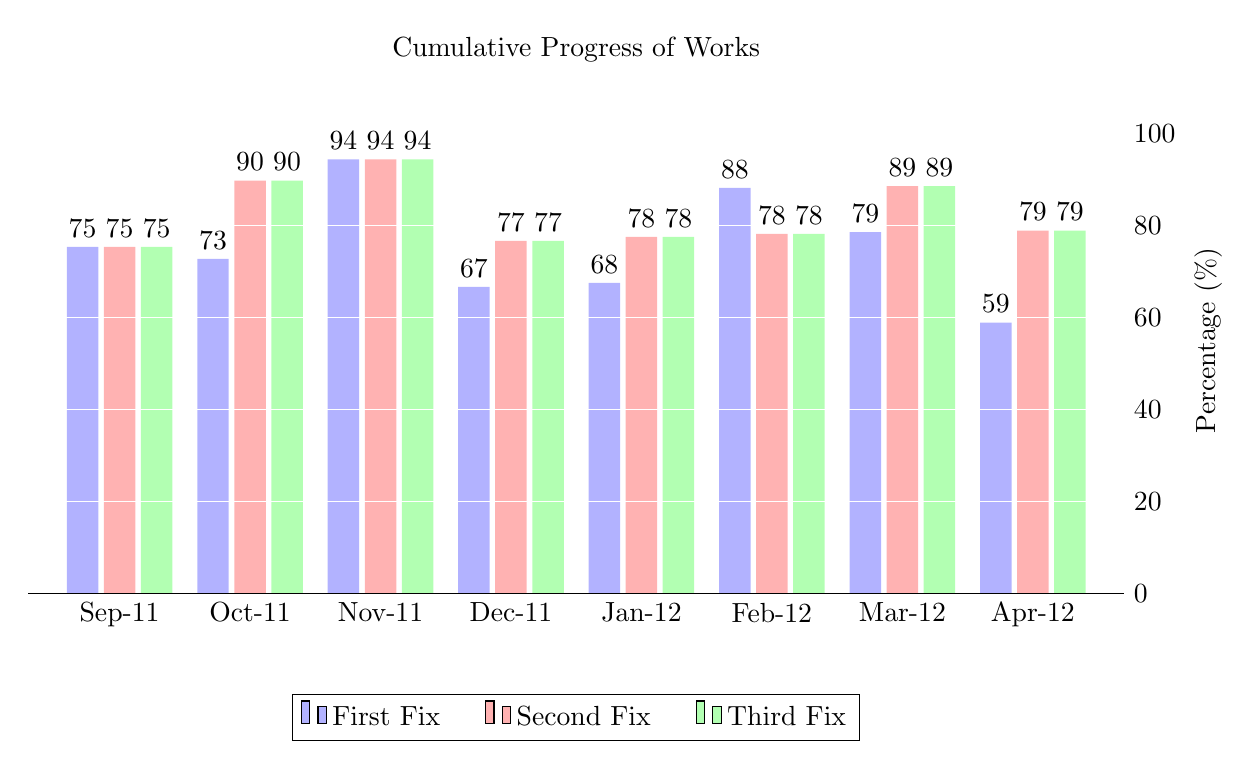
\begin{tikzpicture}
  \centering
  \begin{axis}[
      ybar, axis on top,
      title={Cumulative Progress of Works},
      height=8cm, width=15.5cm,
      bar width=0.4cm,
      ymajorgrids, tick align=inside,
      major grid style={draw=white},
      enlarge y limits={value=.1,upper},
      ymin=0, ymax=100,
      axis x line*=bottom,
      axis y line*=right,
      y axis line style={opacity=0},
      tickwidth=0pt,
      enlarge x limits=true,
      legend style={
        at={(0.5,-0.2)},
        anchor=north,
        legend columns=-1,
        /tikz/every even column/.append style={column sep=0.5cm}
      },
      ylabel={Percentage (\%)},
      symbolic x coords={
        Sep-11,Oct-11,Nov-11,Dec-11,
        Jan-12,Feb-12,
        Mar-12,
        Apr-12
      },
      xtick=data,
      nodes near coords={
        \pgfmathprintnumber[precision=0]{\pgfplotspointmeta}
      }
    ]
    \addplot [draw=none, fill=blue!30] coordinates {
      (Sep-11,75.4064)
      (Oct-11, 72.7961)
      (Nov-11,94.4597)
      (Dec-11,66.6786)
      (Jan-12,67.5600)
      (Feb-12,88.2339)
      (Mar-12,78.6138)
      (Apr-12,58.9129) 
    };
    \addplot [draw=none,fill=red!30] coordinates {
      (Sep-11,75.4064)
      (Oct-11, 89.7961)
      (Nov-11,94.4597)
      (Dec-11,76.6786)
      (Jan-12,77.5600)
      (Feb-12,78.2339)
      (Mar-12,88.6138)
      (Apr-12,78.9129) 
    };
    \addplot [draw=none, fill=green!30] coordinates {
      (Sep-11,75.4064)
      (Oct-11, 89.7961)
      (Nov-11,94.4597)
      (Dec-11,76.6786)
      (Jan-12,77.5600)
      (Feb-12,78.2339)
      (Mar-12,88.6138)
      (Apr-12,78.9129) 
    };
    \legend{First Fix,Second Fix,Third Fix}
  \end{axis}
\end{tikzpicture}

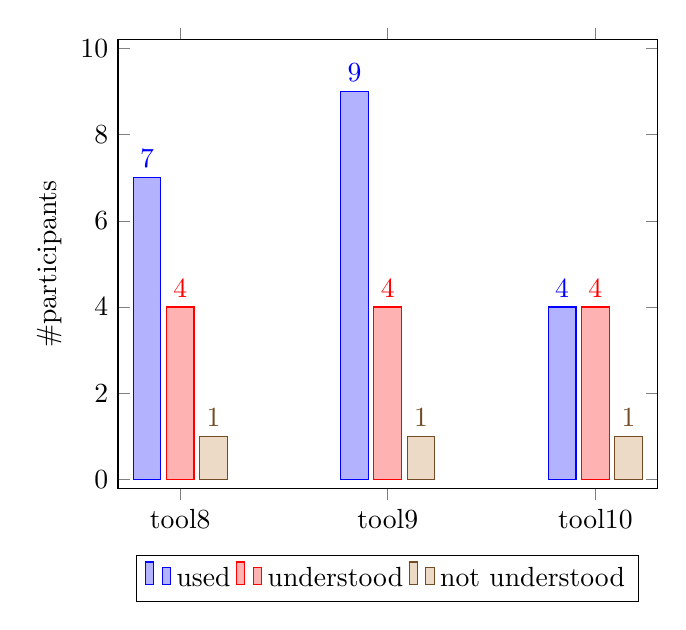
\begin{tikzpicture}
  \begin{axis}[
      ybar,
      enlargelimits=0.15,
      legend style={at={(0.5,-0.15)},
        anchor=north,legend columns=-1},
      ylabel={\#participants},
      symbolic x coords={tool8,tool9,tool10},
      xtick=data,
      nodes near coords,
      nodes near coords align={vertical},
    ]
    \addplot coordinates {(tool8,7) (tool9,9) (tool10,4)};
    \addplot coordinates {(tool8,4) (tool9,4) (tool10,4)};
    \addplot coordinates {(tool8,1) (tool9,1) (tool10,1)};
    \legend{used,understood,not understood}
  \end{axis}
\end{tikzpicture}

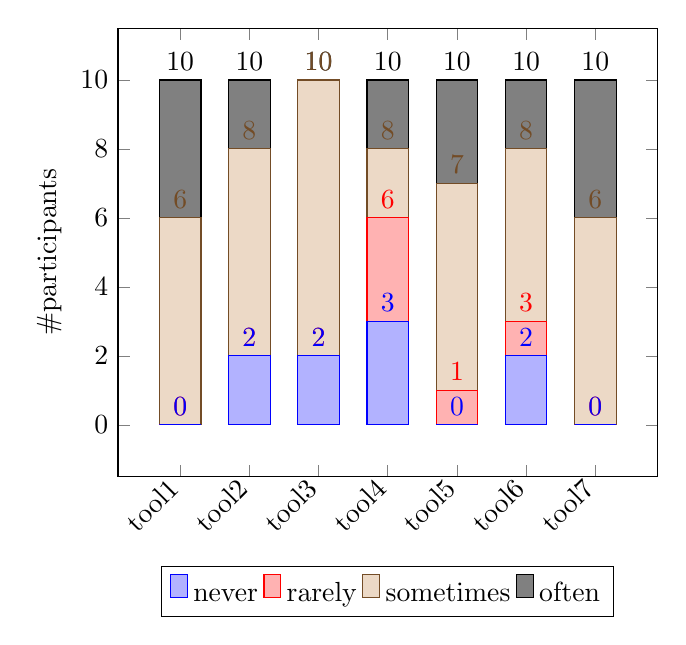
\begin{tikzpicture}
  \begin{axis}[
      ybar stacked,
      bar width=15pt,
      nodes near coords,
      enlargelimits=0.15,
      legend style={at={(0.5,-0.20)},
        anchor=north,legend columns=-1},
      ylabel={\#participants},
      symbolic x coords={tool1, tool2, tool3, tool4,
        tool5, tool6, tool7},
      xtick=data,
      x tick label style={rotate=45,anchor=east},
    ]
    \addplot+[ybar] plot coordinates {(tool1,0) (tool2,2)
      (tool3,2) (tool4,3) (tool5,0) (tool6,2) (tool7,0)};
    \addplot+[ybar] plot coordinates {(tool1,0) (tool2,0)
      (tool3,0) (tool4,3) (tool5,1) (tool6,1) (tool7,0)};
    \addplot+[ybar] plot coordinates {(tool1,6) (tool2,6)
      (tool3,8) (tool4,2) (tool5,6) (tool6,5) (tool7,6)};
    \addplot+[ybar] plot coordinates {(tool1,4) (tool2,2)
      (tool3,0) (tool4,2) (tool5,3) (tool6,2) (tool7,4)};
    \legend{\strut never, \strut rarely, \strut sometimes, \strut often}
  \end{axis}
  \end{tikzpicture}

\end{document}
